\chapter{Introduction}
\label{intro}

\pagenumbering{arabic} 


Action recognition is an active research field, which has received considerable attention in computer vision in the past decade. The major goal of action recognition is to automatically understand different types of actions to reduce human workload. The ever-growing interest in recognizing human actions is in part due to the wide range of applications, including, but not limited to the following:

\noindent
\textbf{Intelligent Visual Surveillance.} There are number of cameras deployed for security surveillance to monitor criminal or suspicious activities, but these require constant human monitoring. To minimize the human workload, intelligent visual surveillance systems can be used to automatically detect and recognize suspicious activities and can generate alerts to security personnel~\cite{xiang2008video} in order to prevent any dangerous situations.
\begin{figure}[!ht]
\begin{center}
	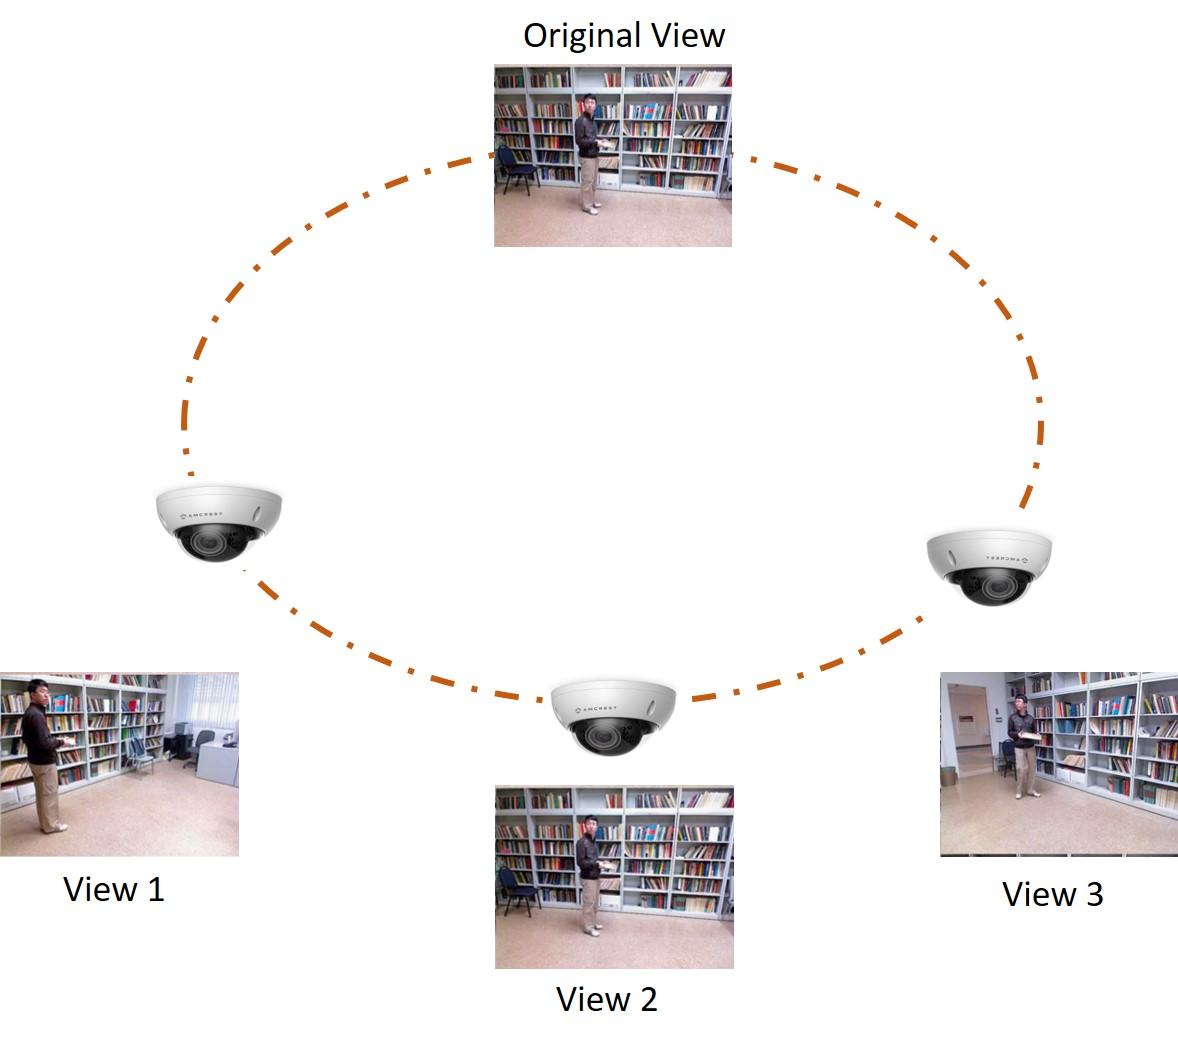
\includegraphics[width=4.5in,height=4in]{figures/motivationfigure.jpg}
	\linebreak
	\captionof{figure}{Illustration of cross-view action recognition in surveillance system.}
	\label{fig1:MEHTODILL}
\end{center}
\end{figure}

\noindent
\textbf{Ambient Assisted Living.} Ambient assisted living systems are used in health care \cite{MUBASHIR2013144} to automatically monitor and analyze patient activities, and also daily life activities especially for elderly people such as falling down, having a stroke or respiration issue, etc.

\noindent
\textbf{Human-computer Interaction.} Human gestures can be used to operate different tasks in the computer such as changing presentation slides using hand gestures instead of using traditional methods such as keyboard and mouse~\cite{799904}.

\noindent
\textbf{Entertainment.} The modern era of gaming uses the human body as a controller instead of using gaming controllers. These systems can be used to track a player's activity during his or her interaction with the gaming environment~\cite{VALLIM20136258}.
%\\
%There are number of action recognition studies have been carried out but it still remains very challenging task, mainly because there is usually large amount of viewpoint variations, different illumination conditions, occlusion, variance in human appearance, shape, clothes, cluttered backgrounds, stationary and moving cameras.\\
%\noindent\textcolor{blue}{

Considerable work is done for single view action recognition when videos are captured from a fixed view using one camera~\cite{sharma2013expanded,liang2013learning,wu2014multi,benmokhtar2014robust,papadopoulos2014real}. However, from the above-mentioned applications, there can be multiple cameras to capture a single action from different viewpoints or angles to get enriched information for action description as shown in Figure~\ref{fig1:MEHTODILL}, where single object actions are captured by three different cameras fixed at three different angles. Most of the proposed approaches  for single view or multi-view action recognition consist of feature engineering which includes different feature extraction~\cite{Efros:2003:RAD:946247.946720,4270156,5459184,wang2013action,1238378}, dictionary learning~\cite{8082519,4483511,zheng2016cross}, and deep learning~\cite{deng2014deep} methods.
However, it is still challenging to recognize action from different view points because the same action looks quite different across views. There are a couple of methods proposed for multi-view or cross-view action recognition, but multiple challenges still remain which need to be addressed~\cite{ji2010advances,holte2011human}.
%\\

The first key step for action recognition is to extract features from video frames. Feature extraction can be understood as a process of retrieving values at the pixel level which is informative and non-redundant. These values give us points of interest which on their own do not contribute to the action itself but extract most relevant points from the raw data. There are challenges in feature extraction, like cluttered images where it is hard to differentiate objects from one another, similarity in colors between objects, camera motion which can bring noise in the images and create blurred frames, large amount of viewpoint variations, different illumination conditions, occlusion, variance in human appearance, shapes, clothes, etc. Another major challenge in this process is selecting a suitable framework that can represent the extracted features accurately and also take into consideration the changes in the spatial and temporal information.
Many feature representation methods are proposed for action recognition in video sequences, such as optical flow patterns~\cite{Efros:2003:RAD:946247.946720,1315182}, shape feature~\cite{4270156,5459184,1211340,4587527}, space-time pattern templates~\cite{1467373,1544882} dense trajectories~\cite{wang2013dense}, improved dense trajectories~\cite{wang2013action}, and spatio-temporal interest points~\cite{1238378}. Although these handcrafted low-level feature methods are powerful to recognize actions in similar view or in controlled scenarios, the performance degrades with viewpoint changes. One reason is appearance difference when observed from different angles, due to this along with view change, the low-level features become less discriminative. One possible solution is brutal-force approach that trains a separate classifier for each view, but it becomes intractable as the number of action categories and views increase. In addition, it is computationally expensive or infeasible to train a separate classifier to address the action under novel views. Another approach is to build view invariant~\cite{10.1007/978-3-540-88688-4_22,6939719,zheng2016cross,zheng2013learning, 7045574, 7907301,6958807} representation for action recognition. 

Although these low-level features achieved great success, designing the effective discriminative features requires the new domain knowledge and these hand-crafted features cannot simply be adapted to new conditions. Learning feature from data itself is considered a plausible way to overcome these limitations and successful examples are dictionary learning and deep learning.
%\\
The idea of deep learning is to discover multiple levels of representation~\cite{deng2014deep}, that deeply learned features will represent the abstract semantics of data. It is expected from deep learning models, that these will provide features which will be more invariant to intra-class variability. The issue with deep learning is that it requires the large amount of labeled data to train a model, and in some cases, it is impossible or not practical. Sometimes pre-trained models are used for feature extraction and then weights of these pre-trained models are fine-tuned. However, the effectiveness of the \enquote{transferred} features becomes worse when source and target become less similar.
 
 %\\
 %\noindent
 In contrast, dictionary learning (DL) methods have demonstrated great success in image classification tasks on both small and large intra-class variation datasets~\cite{8082519}. The last few years have witnessed the fast development of DL methods under sparse representation theory, i.e., signals can be well-approximated by the linear combination of few columns of some basis or dictionary~\cite{4483511}. The dictionary that faithfully and discriminatively encodes signals plays an important role in the success of sparse representation. Conventional dictionary learning performs well for different classification and recognition tasks, but the performance deteriorates for cross-view action recognition. The primary reason is discriminative features for each view are not in common feature subspace. Notably, there are view-shared sparse representation based approaches proposed~\cite{zheng2013learning,zheng2016cross}. In those approaches, they assumed that different views contribute equally in shared features, and they ignored view-private features, however, it is not always valid.  
 
 Another approach is to incorporate transfer learning to bring the source and target in the common subspace. Transfer learning aims to improve the learning of target predictive function using the source knowledge.
Transfer learning tries to bring the distribution of source and target domain in the common subspace by learning knowledge from one or more source domains and transfer that to target domain in order to improve the performance~\cite{Weiss2016}.
The main purpose is to find the common representative for the similar objects which look different when they are in different views.

% Transfer learning definition
 Transfer learning can be performed in supervised, semi-supervised and unsupervised ways. In supervised learning~\cite{daume2009frustratingly, chattopadhyay2012multisource} the source and target both contain labeled data, in semi-supervised~\cite{chattopadhyay2012multisource,blitzer2006domain1} source domain has labeled data, while target domain has limited or no labeled data, and in unsupervised~\cite{cook2013transfer} there is no labeled data for both source and target domains. In brief, transfer learning may help to improve the performance for cross-view action recognition, but with performance being compromised, because source and target may not be discriminative in common space.   

\section{Motivation}
Considerable feature representation methods have been proposed for action recognition in videos, but these are only powerful for same view action recognition. In that sense, the performance degrades when the same action is performed from a different view. Recent learning approaches have cast a light on such issues. First, transfer learning or domain adaptation methods have shown good results for such scenarios, but this approach is largely limited by discriminant ability because the features brought up in the common subspace neither promotes the underlying sparse structure of data, nor preserve the best features. Second, shared dictionary learned for cross-view action recognition provides sparse representation, but it may ignore view private features. In some cases, e.g., when actions are performed from unseen views which are not part of the shared dictionary, the performance will degrade significantly.

Motivated by the above analysis and the limitation of transfer learning and dictionary learning for cross-view action recognition when these methods are incorporated separately, we proposed a novel approach called \textbf{Joint Dictionary and Transfer Learning (JDTL)} that helps to improve the performance of cross-view action recognition, where dictionary learning pursues the discriminative and robust representation for each view and transfer learning aims to bring those discriminative features of each view in the common subspace.
\newpage
\section{Contribution}
The main technical contributions of this work are:
\begin{itemize}
\item We pursue discriminant dictionary learning in each view with $D^{(v)}$ as the $v$-th view dictionary and  $X^{(v)}$ as the coding and we learned view independent dictionaries $D^{(v)} = [D_1^{(v)},D_2^{(v)},\cdots,D_C^{(v)}]$ to extract discriminative features for $C$ different actions. A common feature space will be optimized through transfer learning across different views in a joint learning framework with dictionary learning.
\item An iterative optimization is developed to approach our learning problems where the transfer learning projection matrix $P$, dictionary $D$ and coefficients $X$ are learned simultaneously. In each iteration, the coefficients $X$ are updated by fixing $P$ and $D$, dictionary $D$ is refined by fixing the $P$ and $X$, and $P$ is learned by fixing $D$ and $X$. The learning process will terminate until the objective converges.
\item To evaluate the proposed method, extended experiments have been performed on PKU-MMD dataset~\cite{liu2017pku}, a benchmark multi-view action recognition dataset. Experimental results demonstrate that our proposed method has achieved promising results for cross-view action recognition.
\end{itemize}

% 1). We introduce $D^{(v)}$ as the v-th view dictionary and  $X^{(v)}$ as the v-th coding and we learned view independent dictionaries $D^{(v)} = [D_1^{(v)},D_2^{(v)},\cdots,D_C^{(v)}]$ to extract discriminative features for $C$ actions. 
% %The main contribution of our work is given in two-folds. First, the success of dictionary learning inspires us to learn view-independent dictionaries for each view. 
% 2)These discriminative features are projected in common subspace through transfer learning across different views.}\\
% \noindent
% Our proposed method is an iterative process where the transfer learning projection matrix $P$, dictionary $D$ and coefficients $X$ are learned simultaneously. In each iteration, the coefficients $X$ are updated by fixing $P$ and $D$, and refines the dictionary $D$ by fixing the $P$ and $X$, while $P$ is learned by fixing $D$ and $X$. The aim is to get optimized projection matrix $P$, dictionary $D$ and coefficients $X$. \\
% \noindent
% To evaluate the proposed method, an extended experimentation is performed on PKU-MMD dataset~\cite{liu2017pku}, a benchmark multi-view action recognition dataset.\ Experimental results demonstrate that our proposed method has achieved significant results for cross-view action recognition. 
\section{Outline}
This thesis consists of 6 chapters including the introduction. Chapter 2 reviews the recent work. Chapter 3 presents the proposed joint dictionary and transfer learning method. Dataset preprocessing and experimental setup are described in Chapter 4. Experimental results and evaluation of our method are discussed in Chapter 5 and we present future work and draw the conclusion in Chapter 6.  






